\documentclass[11pt, letterpaper]{article}
\usepackage[margin=1.5cm]{geometry}
\pagestyle{plain}

\usepackage{amsmath, amsfonts, amssymb, amsthm}
\usepackage[shortlabels]{enumitem}
\usepackage[makeroom]{cancel}
\usepackage{graphicx}
\graphicspath{{./images/}}

\begin{document}
\title{Final Reflection: Proof Writing\\\normalsize MATH311}
\author{Connor Braun}

\allowdisplaybreaks

\maketitle\

\section*{Topic 1}
\begin{center}    
    \makebox[\textwidth]{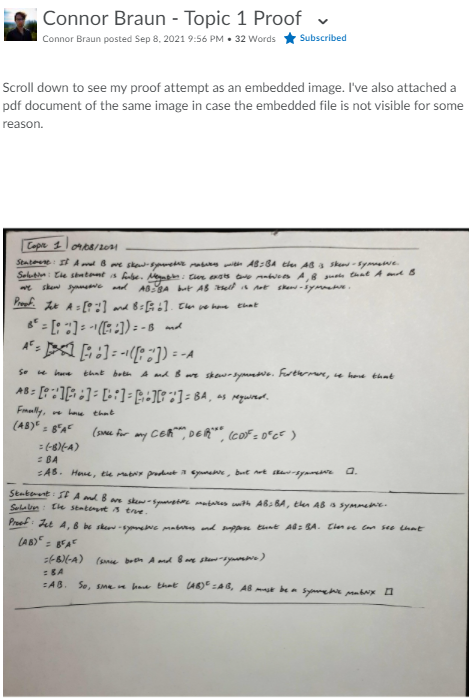
\includegraphics[width=118mm]{topic1_proof}}
\end{center}
\begin{center}    
    \makebox[\textwidth]{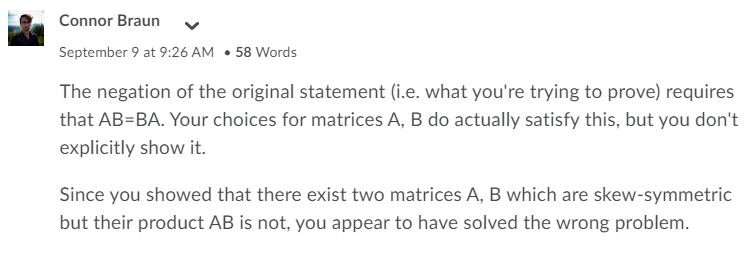
\includegraphics[width=120mm]{topic1_reply1}}
\end{center}
\begin{center}    
    \makebox[\textwidth]{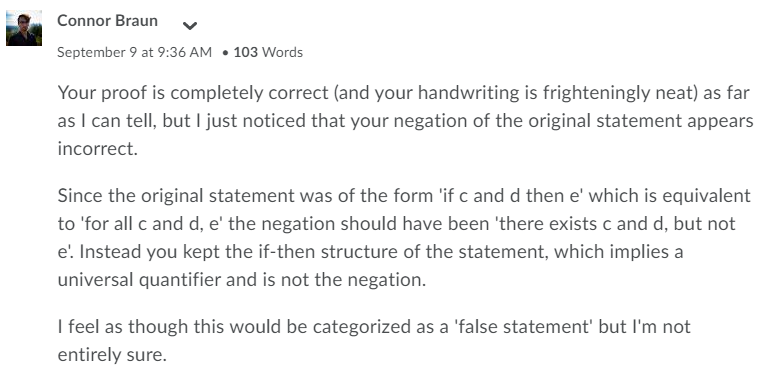
\includegraphics[width=120mm]{topic1_reply2}}
\end{center}
\subsection*{Topic 1 reflection}
Looking back now, I'm happy with this proof and believe it to be correct, but one thing does stand out.\\ 
As a matter of trying to form good proof writing habits, I try to use plain English since it's very easy to overdo the symbolic notation 
and muddy the readability of the proof. However, this approach benefits from 'good writing', which is a major goal of mine -- even though it's a bit nebulous. 
Despite this, one comment from a classmate was essentially to reduce my usage of the phrase: 'we have that...', which is a good suggestion since I habitually use this phrase
often enough to detract from the prose -- 5 times in just this one proof! What's worse is that I {\it still} do this, and
I haven't actually been mindful of it until just now while writing this reflection. I'll try to vary my language going forward,
and also take this as an opportunity to work on forming a cohesive narrative; at least when writing longer proofs.   
\newpage
\section*{Topic 2}
\begin{center}    
    \makebox[\textwidth]{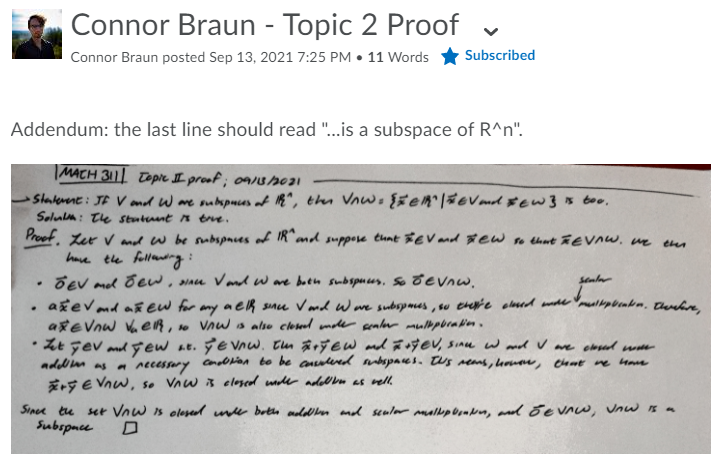
\includegraphics[width=120mm]{topic2_proof}}
\end{center}
\begin{center}    
    \makebox[\textwidth]{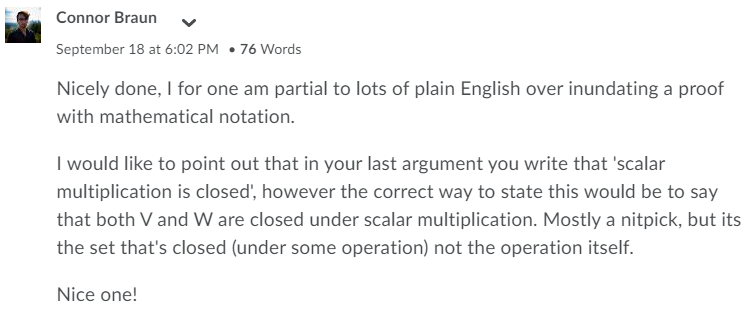
\includegraphics[width=120mm]{topic2_reply1}}
\end{center}
\begin{center}    
    \makebox[\textwidth]{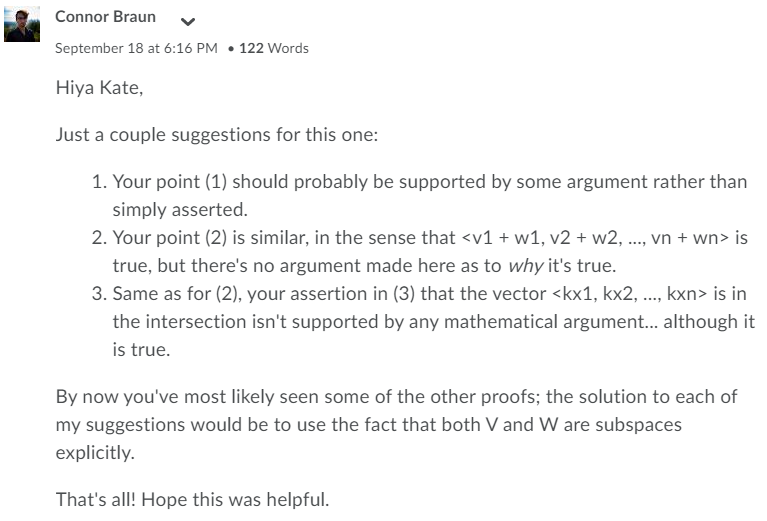
\includegraphics[width=120mm]{topic2_reply2}}
\end{center}
\subsection*{Topic 2 reflection}
I remember this proof feeling straightforward at the time of my writing it, and even now it strikes me as 
concise, clear and correct. One suggestion from a peer was to improve the prose by introducing variables as I use them
rather than at the outset of the proof. Upon reflection I actually disagree with their comment, since then if a reader 
wanted to revisit the definition of some variable they would have to scan the body of the writing rather than simply 
direct their attention to the top. My colleague's suggestion isn't without merit; introducing variables as they're 
used means that the reader wouldn't have to disrupt their reading to revisit the variable's definition elsewhere. I 
choose to disregard their suggestion on the grounds that reading proofs usually consists of a lot of pausing and 
thinking, so there is little benefit to scattering my variable definitions so that the more advanced reader needn't 
lift their eyes from the page. 
\newpage
\section*{Topic 3}
\begin{center}    
    \makebox[\textwidth]{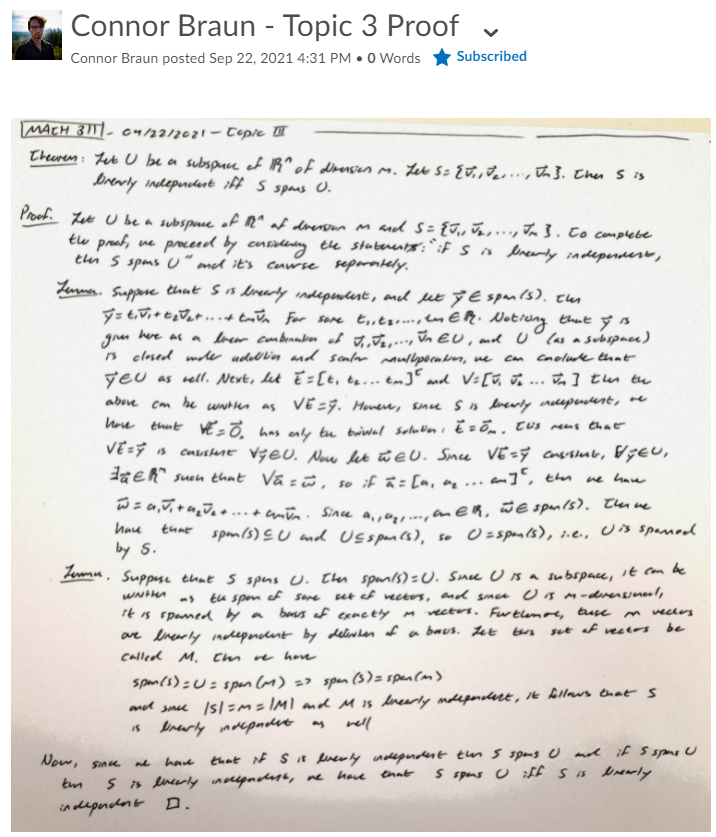
\includegraphics[width=120mm]{topic3_proof}}
\end{center}
\begin{center}    
    \makebox[\textwidth]{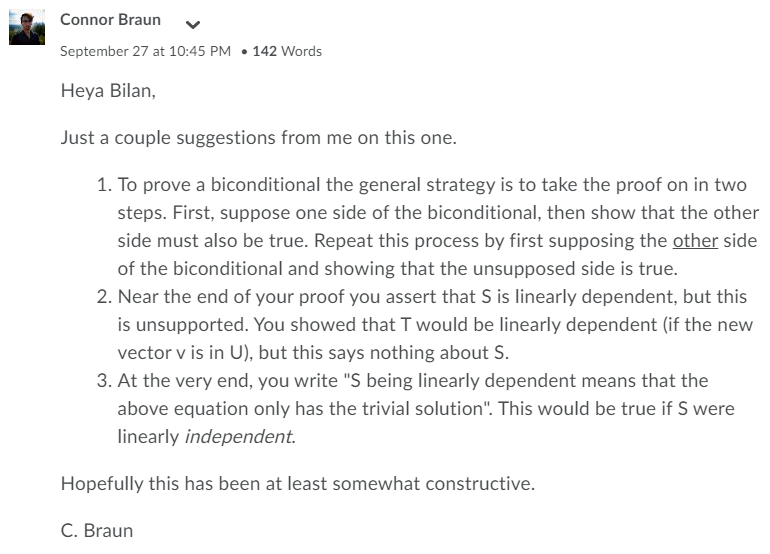
\includegraphics[width=120mm]{topic3_reply1}}
\end{center}
\begin{center}    
    \makebox[\textwidth]{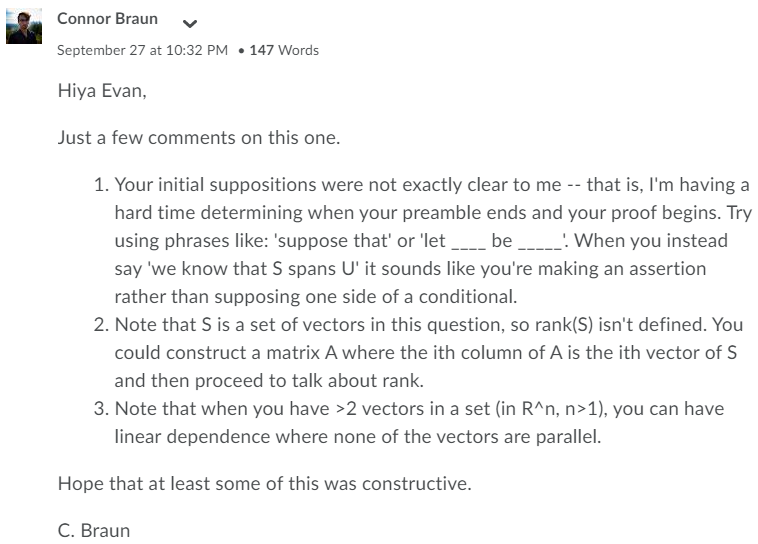
\includegraphics[width=120mm]{topic3_reply2}}
\end{center}
\subsection*{Topic 3 reflection}
This proof took me the longest to write of any of the 5 I chose to complete. Furthermore, it's actually incorrect
since I assume that linear independence of the columns of a matrix make it invertible. This holds for square 
matrices, but the suppositions here do not preclude the possibility of a nonsquare matrix, for which this result
does not hold. Perhaps more importantly, however, was the approach I took and the reason for it. This proof 
is a bit tricky, and my general inclination when dealing with tricky concepts in linear algebra is to try and
formulate the problem as a system of linear equations, with which I'm more comfortable. The problem I've 
found with this approach is that it is not a good default strategy since it often does not lend any clarity 
to the problem at hand and can be quite verbose. I recognized this around the time of submitting this proof, and have
since taken any inclination to form a system of equations as an indication that I had ought review the relevant
concepts for a more direct solution.  
\newpage
\section*{Topic 4}
\begin{center}    
    \makebox[\textwidth]{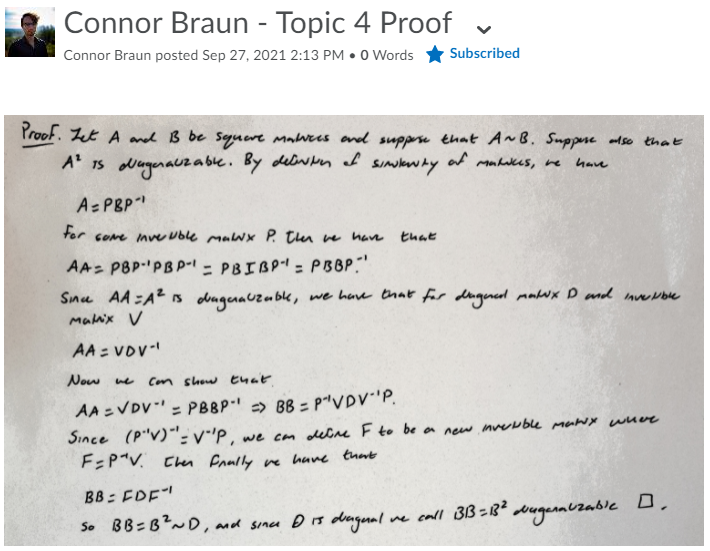
\includegraphics[width=120mm]{topic4_proof}}
\end{center}
\begin{center}    
    \makebox[\textwidth]{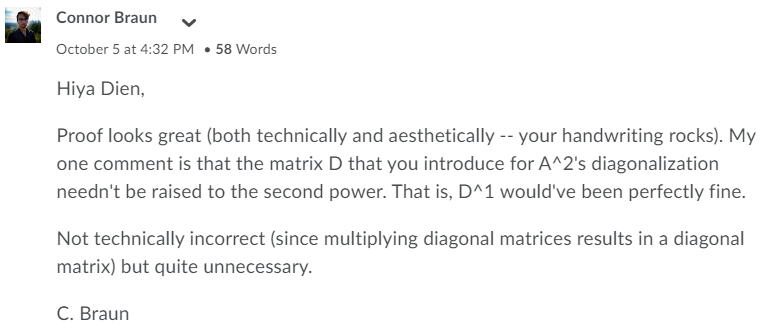
\includegraphics[width=120mm]{topic4_reply1}}
\end{center}
\begin{center}    
    \makebox[\textwidth]{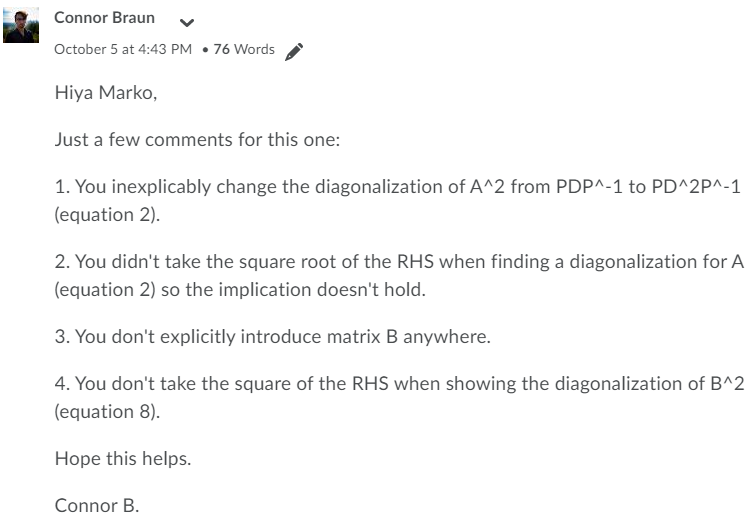
\includegraphics[width=120mm]{topic4_reply2}}
\end{center}
\subsection*{Topic 4 reflection}
I like this proof and think it's correct, but there are two salient points I've gleaned from my reflection on it.
First is that while I thought some symbolic manipulations were clear enough to afford me an implication arrow,
a colleague actually found that this interrupted their interpretation of my work. This makes for a good reminder on
how biased the writer can be as to the readability of a proof -- next time I think that an implication arrow
might suffice I'll default to a one sentence explanation instead.

Secondly, I actually collaborated with a colleage in person to discuss our approach for this proof. This
made for a very productive conversation, and I remember we even proved some only tangentially-related statements
out of curiosity (for example, I believe we proved that all diagonal and symmetric matrices are diagonalizable). 
In light of the pandemic (and the apparent reclusiveness of math majors in general) I rarely get to collaborate
on anything in mathematics. I loved this experience and have made more of an effort to rally classmates 
in all of my math classes since then (within the constraints of academic integrity, of course). 
\newpage
\section*{Topic 5}
\begin{center}    
    \makebox[\textwidth]{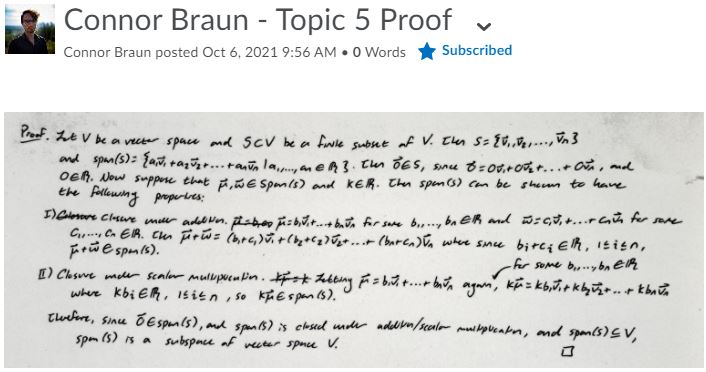
\includegraphics[width=120mm]{topic5_proof}}
\end{center}
\begin{center}    
    \makebox[\textwidth]{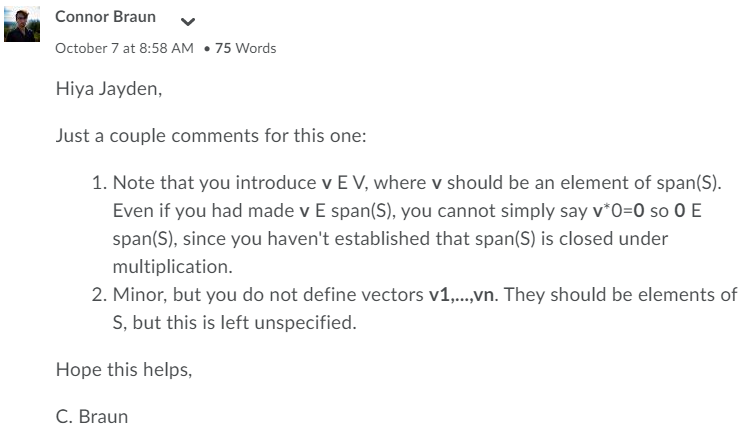
\includegraphics[width=120mm]{topic5_reply1}}
\end{center}
\begin{center}    
    \makebox[\textwidth]{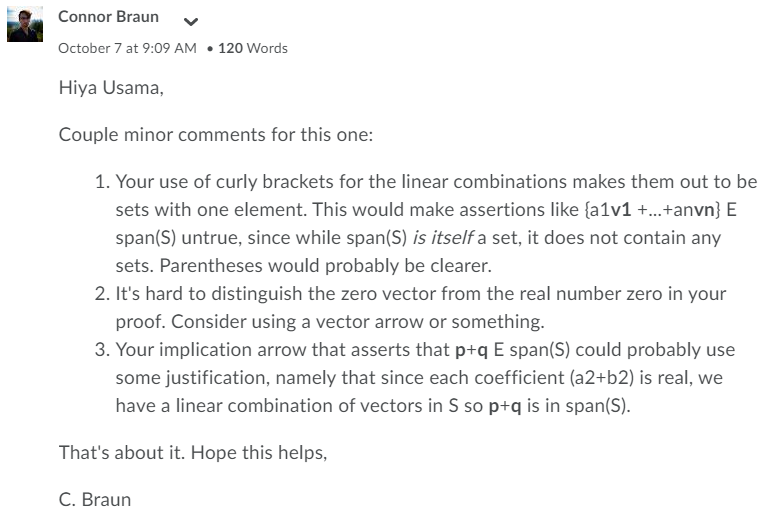
\includegraphics[width=120mm]{topic5_reply2}}
\end{center}
\subsection*{Topic 5 reflection}
Upon reflection, I like this proof and think it's both concise and correct. One problem I recall encountering
was that I actually scrapped and rewrote the thing some two or three times. The reason for this
was that the prompt struck me as fairly straightforward, so instead of planning my approach on a scratchpad
beforehand I simply dived into writing the final draft. Despite rewriting it a few times, there are many
little mistakes which have been crossed out and corrected in the margins, which makes for a messy read.
For me this is a dead giveaway that I didn't think ahead before writing (and a common feature of every
math test I've ever written) and is a good reminder to not proceed so boldly -- time permitting.





\end{document}